% Soubory musí být v kódování, které je nastaveno v příkazu \usepackage[...]{inputenc}

\documentclass[%
%  draft,    				  % Testovací překlad
  12pt,       				% Velikost základního písma je 12 bodů
  a4paper,    				% Formát papíru je A4
%  oneside,      			% Jednostranný tisk (výchozí)
%% Z následujicich voleb lze použít maximálně jednu:
%	dvipdfm  						% výstup bude zpracován programem 'dvipdfm' do PDF
%	dvips	  						% výstup bude zpracován programem 'dvips' do PS
%	pdftex							% překlad bude proveden programem 'pdftex' do PDF (výchozí)
	unicode,						% Záložky a informace budou v kódování unicode
%% Z následujících voleb lze použít jen jednu:
%english,            % originální jazyk je angličtina
czech              % originální jazyk je čeština (výchozí)
%slovak,             % originální jazyk je slovenčina
]{report}				    	% Dokument třídy 'zpráva'

\usepackage[utf8]		%	Kódování zdrojových souborů je v UTF-8
	{inputenc}					% Balíček pro nastavení kódování zdrojových souborů

\usepackage{graphicx} % Balíček 'graphicx' pro vkládání obrázků
											% Nutné pro vložení log školy a fakulty

\usepackage[
	nohyperlinks				% Nebudou tvořeny hypertextové odkazy do seznamu zkratek
]{acronym}						% Balíček 'acronym' pro sazby zkratek a symbolů
											% Nutné pro použití prostředí 'seznamzkratek' balíčku 'thesis'

\usepackage[
	breaklinks=true,		% Hypertextové odkazy mohou obsahovat zalomení řádku
	hypertexnames=false % Názvy hypertextových odkazů budou tvořeny
											% nezávisle na názvech TeXu
]{hyperref}						% Balíček 'hyperref' pro sazbu hypertextových odkazů
											% Nutné pro použití příkazu 'nastavenipdf' balíčku 'thesis'

\usepackage{pdfpages} % Balíček umožňující vkládat stránky z PDF souborů
                      % Nutné při vkládání titulních listů a zadání přímo
                      % ve formátu PDF z informačního systému

\usepackage{enumitem} % Balíček pro nastavení mezerování v odrážkách
  \setlist{topsep=0pt,partopsep=0pt,noitemsep}

\usepackage{cmap} 		% Balíček cmap zajišťuje, že PDF vytvořené `pdflatexem' je
											% plně "prohledávatelné" a "kopírovatelné"

\usepackage{upgreek}	% Balíček pro sazbu stojatých řeckých písmem
											% např. stojaté pí: \uppi
											% např. stojaté mí: \upmu (použitelné třeba v mikrometrech)
											% pozor, grafická nekompatibilita s fonty typu Computer Modern!

\usepackage{dirtree}		% sazba adresářové struktury

\usepackage[formats]{listings}	% Balíček pro sazbu zdrojových textů
\lstset{
%	Definice jazyka použitého ve výpisech
%    language=[LaTeX]{TeX},	% LaTeX
%	language={Matlab},		% Matlab
	language={C},           % jazyk C
    basicstyle=\ttfamily,	% definice základního stylu písma
    tabsize=2,			% definice velikosti tabulátoru
    inputencoding=utf8,         % pro soubory uložené v kódování UTF-8
    %inputencoding=cp1250,      % pro soubory uložené ve standardním kódování Windows CP1250
		columns=fixed,  %flexible,
		fontadjust=true %licovani sloupcu
    extendedchars=true,
    literate=%  definice symbolů s diakritikou
    {á}{{\'a}}1
    {č}{{\v{c}}}1
    {ď}{{\v{d}}}1
    {é}{{\'e}}1
    {ě}{{\v{e}}}1
    {í}{{\'i}}1
    {ň}{{\v{n}}}1
    {ó}{{\'o}}1
    {ř}{{\v{r}}}1
    {š}{{\v{s}}}1
    {ť}{{\v{t}}}1
    {ú}{{\'u}}1
    {ů}{{\r{u}}}1
    {ý}{{\'y}}1
    {ž}{{\v{z}}}1
    {Á}{{\'A}}1
    {Č}{{\v{C}}}1
    {Ď}{{\v{D}}}1
    {É}{{\'E}}1
    {Ě}{{\v{E}}}1
    {Í}{{\'I}}1
    {Ň}{{\v{N}}}1
    {Ó}{{\'O}}1
    {Ř}{{\v{R}}}1
    {Š}{{\v{S}}}1
    {Ť}{{\v{T}}}1
    {Ú}{{\'U}}1
    {Ů}{{\r{U}}}1
    {Ý}{{\'Y}}1
    {Ž}{{\v{Z}}}1
}

%% Nastavení českého jazyka při sazbě v češtině.
% Pro sazbu češtiny je možné použít mezinárodní balíček 'babel', jenž
% použití doporučujeme pro nové instalace (MikTeX2.8,TeXLive2009), nebo
% národní balíček 'czech', který doporučujeme ve starších instalacích.
% Balíček 'babel' bude správně fungovat pouze ve spojení s programy
% 'latex', 'pdflatex', zatímco balíček 'czech' bude fungovat ve spojení
% s programy 'cslatex', 'pdfcslatex'.
% Varianta A:
\usepackage    				
  {babel}             % Balíček pro sazbu různojazyčných dokumentů; kompilovat (pdf)latexem!
  										% převezme si z parametrů třídy správný jazyk
\usepackage{lmodern}	% vektorové fonty Latin Modern, nástupce půvoních Knuthových Computern Modern fontů
\usepackage{textcomp} % Dodatečné symboly
\usepackage[T1]{fontenc}  % Kódování fontu - mj. kvůli správným vzorům pro dělení slov
% Varianta B:
%\usepackage{czech}   % Alternativní balíček pro sazbu v českém jazyce, kompilovat (pdf)cslatexem!

\usepackage[%
%% Z následujících voleb lze použít pouze jednu
% left,               % Rovnice a popisky plovoucich objektů budou %zarovnány vlevo
  center,             % Rovnice a popisky plovoucich objektů budou zarovnány na střed (vychozi)
%% Z následujících voleb lze použít pouze jednu
semestral						%	sazba zprávy semestrálního projektu
%bachelor						%	sazba bakalářské práce
%diploma						 % sazba diplomové práce
%treatise            % sazba pojednání o dizertační práci
%phd                 % sazba dizertační práce
]{thesis}             % Balíček pro sazbu studentských prací
                      % Musí být vložen až jako poslední, aby
                      % ostatní balíčky nepřepisovaly jeho příkazy
\usepackage{caption}
\usepackage{placeins}
\usepackage{url}
\DeclareUrlCommand\url{\def\UrlLeft{<}\def\UrlRight{>} \urlstyle{tt}}  
                      
%%%%%%%%%%%%%%%%%%%%%%%%%%%%%%%%%%%%%%%%%%%%%%%%%%%%%%%%%%%%%%%%%
%%%%%%      Definice informací o dokumentu             %%%%%%%%%%
%%%%%%%%%%%%%%%%%%%%%%%%%%%%%%%%%%%%%%%%%%%%%%%%%%%%%%%%%%%%%%%%%

%% Název práce:
%  První parametr je název v originálním jazyce,
%  druhý je překlad v angličtině nebo češtině (pokud je originální jazyk angličtina)
\nazev{Programový modul pro zobrazení mračna bodů ve virtuální realitě}{Software Module for Point Clouds Display in Virtual Reality}

%% Jméno a příjmení autora ve tvaru
%  [tituly před jménem]{Křestní}{Příjmení}[tituly za jménem]
\autor[]{Martin}{Bařinka}

%% Jméno a příjmení vedoucího včetně titulů
%  [tituly před jménem]{Křestní}{Příjmení}[tituly za jménem]
% Pokud vedoucí nemá titul za jménem, smažte celý řetězec '[...]'
\vedouci[prof.\ Ing.]{Luděk}{Žalud}[Ph.D.]

%% Jméno a příjmení oponenta včetně titulů
%  [tituly před jménem]{Křestní}{Příjmení}[tituly za jménem]
% Pokud nemá titul za jménem, smažte celý řetězec '[...]'
% Uplatní se pouze v prezentaci k obhajobě
%\oponent{}{}

%% Označení oboru studia
% První parametr je obor v originálním jazyce,
% druhý parametr je překlad v angličtině nebo češtině
%\oborstudia{Teleinformatika}{Teleinformatics}

%% Označení ústavu
% První parametr je název ústavu v originálním jazyce,
% druhý parametr je překlad v angličtině nebo češtině
\ustav{Ústav automatizace a měřicí techniky}{Department of Control and Instrumentation} 

%% Rok obhajoby
\rok{Rok}
\datum{10.\,1.\,2017} % Uplatní se pouze v prezentaci k obhajobě

%% Místo obhajoby
% Na titulních stránkách bude automaticky vysázeno VELKÝMI písmeny
\misto{Brno}

%% Abstrakt
\abstrakt{Cílem práce bylo seznámit se s hardwarem a softwarem zařízení pro virtuální realitu, prozkoumat možnosti vývoje a navržením softwarového řešení pro zobrazování medicínských dat, z CT, MRI nebo RoScan vyvíjeným na VUT. }{The goal of my task was to understand hardware and software of equipment for virtual reality, investigate possibilities to develop and design software solution for medical dates from CT, MRI or RoScan, developed at VUT.}

%% Klíčová slova
\klicovaslova{Virtuální realita; mračna bodů; mesh; 3D zobrazování}%
	{Virtual reality; pointcloud; mesh; 3D rendering}

%% Poděkování
\podekovanitext{Rád bych poděkoval vedoucímu diplomové práce panu prof. Ing. Luděk Žalud Ph.D.\ za odborné vedení, konzultace, trpělivost a podnětné návrhy k~práci.}  % do tohoto souboru doplňte údaje o sobě, o názvu práce...

%%%%%%%%%%%%%%%%%%%%%%%%%%%%%%%%%%%%%%%%%%%%%%%%%%%%%%%%%%%%%%%%%%%%%%%%

%%%%%%%%%%%%%%%%%%%%%%%%%%%%%%%%%%%%%%%%%%%%%%%%%%%%%%%%%%%%%%%%%%%%%%%%
%%%%%%     Nastavení polí ve Vlastnostech dokumentu PDF      %%%%%%%%%%%
%%%%%%%%%%%%%%%%%%%%%%%%%%%%%%%%%%%%%%%%%%%%%%%%%%%%%%%%%%%%%%%%%%%%%%%%
%% Při vloženém balíčku 'hyperref' lze použít příkaz '\nastavenipdf'
\nastavenipdf
%  Nastavení polí je možné provést také ručně příkazem:
%\hypersetup{
%  pdftitle={Název studentské práce},    	% Pole 'Document Title'
%  pdfauthor={Autor studenstké práce},   	% Pole 'Author'
%  pdfsubject={Typ práce}, 						  	% Pole 'Subject'
%  pdfkeywords={Klíčová slova}           	% Pole 'Keywords'
%}
%%%%%%%%%%%%%%%%%%%%%%%%%%%%%%%%%%%%%%%%%%%%%%%%%%%%%%%%%%%%%%%%%%%%%%%

%%%%%%%%%%%%%%%%%%%%%%%%%%%%%%%%%%%%%%%%%%%%%%%%%%%%%%%%%%%%%%%%%%%%%%%
%%%%%%%%%%%       Začátek dokumentu               %%%%%%%%%%%%%%%%%%%%%
%%%%%%%%%%%%%%%%%%%%%%%%%%%%%%%%%%%%%%%%%%%%%%%%%%%%%%%%%%%%%%%%%%%%%%%
\begin{document}


%% Vložení desek generovaných informačním systémem
\includepdf[pages=1,offset=19mm 0mm]%
  {pdf/desky}% název souboru nesmí obsahovat mezery!
% nebo vytvoření desek z balíčku
%\vytvorobalku
\setcounter{page}{1} %resetovani citace stranek - desky se necisluji

%% Vložení titulního listu generovaného informačním systémem
\includepdf[pages=1,offset=19mm 0mm]%
  {pdf/TitulniList_color}% název souboru nesmí obsahovat mezery!
% nebo vytvoření titulní stránky z balíčku
%\vytvortitulku
   
%% Vložení zadání generovaného informačním systémem
\includepdf[pages=1,offset=19mm 0mm]%
  {pdf/zadani}% název souboru nesmí obsahovat mezery!
% nebo lze vytvořit prázdný list příkazem ze šablony
%\stranka{}%
%	{\sffamily\Huge\centering ZDE VLOŽIT LIST ZADÁNÍ}%
%	{\sffamily\centering Z~důvodu správného číslování stránek}

%% Vysázení stránky s abstraktem
\vytvorabstrakt

%% Vysázení prohlaseni o samostatnosti
\vytvorprohlaseni

%% Vysázení poděkování
\vytvorpodekovani

%% Vysázení poděkování projektu SIX
% ----------- zakomentujte pokud neodpovida realite
%\vytvorpodekovaniSIX

%% Vysázení obsahu
\obsah

%% Vysázení seznamu obrázků
\seznamobrazku

%% Vysázení seznamu tabulek
%\seznamtabulek

%% Vysázení seznamu výpisů
%\lstlistoflistings

%% Vložení souboru 'text/uvod.tex' s úvodem
\chapter*{Úvod}
\phantomsection
\addcontentsline{toc}{chapter}{Úvod}

Cílem práce je seznámit se s hardwarem i softwarem zařízení pro virtuální realitu, prověřit možnosti vývoje a navržení softwarového řešení pro zobrazování medicínských dat, jako například CT, MRI a RoScan, který je vyvíjen na VUT.

Práce byla zadána mým vedoucím a zaujala mě,  přestože jsem doposud o tomto tématu nic nevěděl a veškeré teoretické informace musím čerpat z internetu. 

V rámci mé práce jsou vstupní data ve formě  mračna bodů nebo meshe a úkolem této práce je zpracovat program, nebo alespoň základ, který bude schopen mračno bodů načíst a zobrazit v helmě virtuální reality.
Prvním úkolem bude vyhledání informací na internetu o technologiích virtuální reality, způsobech vývoje aplikací, datových formátech a vývoji 3D aplikace.

Poté musím vybrat vhodné knihovny a vhodný datový formát tak, aby má aplikace mohla fungovat s mě dostupným headsetem HTC Vive a aby byl datový formát kompatibilní s již používanými programy.

Díky tomuto programu bude moct uživatel vidět zobrazené data jako plastický obraz, což v medicíně může umožnit zkvalitnění diagnostiky. 

%% Vložení souboru 'text/reseni' s popisem reseni práce
\chapter{Teoretická část studentské práce}

\section{Virtuální realita}

Virtuální realita (VR) je technologie, umožňující uživateli interagovat se simulovaným prostředím. Jde o vytváření vizuálního, sluchového, hmatového či jiného vjemu, budícího subjektivní dojem skutečnosti pomocí počítače, speciální audiovizuální helmy, brýlí popřípadě obleku.

\subsection{Stereoskopie}

Za nejjednodušší VR se dá považovat stereoskopie, což je technika vytváření 3D vjemu pomocí dvou 2D obrazů.


Stereoskopie využívá přirozené vlastnosti člověka, tzv. binokulárního vidění. To znamená, že se obrazy vnímané simultánně oběma očima spojí v jeden a navíc nám umožňuje vnímat hloubku prostoru. Každé oko vidí obraz mírně posunutý a mozek poté vytvoří na základě těchto vjemů 3D obraz. Existuje určité procento lidí, u kterých tato schopnost není vyvinuta a ti nejsou schopni správně 3D obraz vidět.


Tradiční stereoskopie vytváří 3D iluzi pomocí dvou 2D obrazů, s různými perspektivami téhož objektu, které se příliš neliší od toho, co by oči přirozeně viděly. Tím vlastně donutí mozek tyto dva rozdílné obrazy zpracovat jako v realitě a mozek vytvoří iluzi prostorového vidění.




\subsubsection{Anaglyf}

Je to technika, která nám umožňuje vytvářet stereoskopický obraz. Obraz pro každé oko je na tomtéž displeji, ale je v opačném odstínu, typicky červené a azurové. Pozorovatel má pak brýle, které mají barevné filtry a tak každé oko vidí pouze jeden z obrazů.

Nevýhodou tohoto řešení je ztráta barevné informace, protože pomocí ní je zakódovaná hloubka obrazu.

\subsubsection{Polarizace}

Další způsob zobrazení stereo obrazu je pomocí polarizačních brýlí. Tyto brýle mají polarizaci jednoho oka kolmou proti druhému. Obraz se pak zobrazuje nebo promítá střídavě přes dvě polarizační skla a brýle pak tyto obrazy odseparují.

Nevýhodou tohoto řešení je nedokonalá polarizace, která plně neodfiltruje druhý obraz a tak vznikají artefakty v obraze.

\subsubsection{Aktivní zatmívací brýle}

Tento způsob pracuje na principu multiplexování. Brýle, synchronně s displejem nebo projektorem, střídavě přepínají obraz pro obě oči.

Nevýhodou tohoto způsobu je velká cena.

\subsubsection{LCD brýle}

Toto jsou brýle, které mají 2 displeje, na které se promítají jednotlivé obrazy. Tyto brýle nemění svůj obraz při pohybu hlavou, jsou vhodné například pro 3D filmy. Brýle, které podporují sledování pohybu se řadí již do headsetů.

Nevýhodou této technologie je vysoká cena, zahřívání a nutné propojení kabelem.

\subsection{Headsety Virtuální reality}

\subsubsection{VFX1}

\begin{figure}
	\centering
	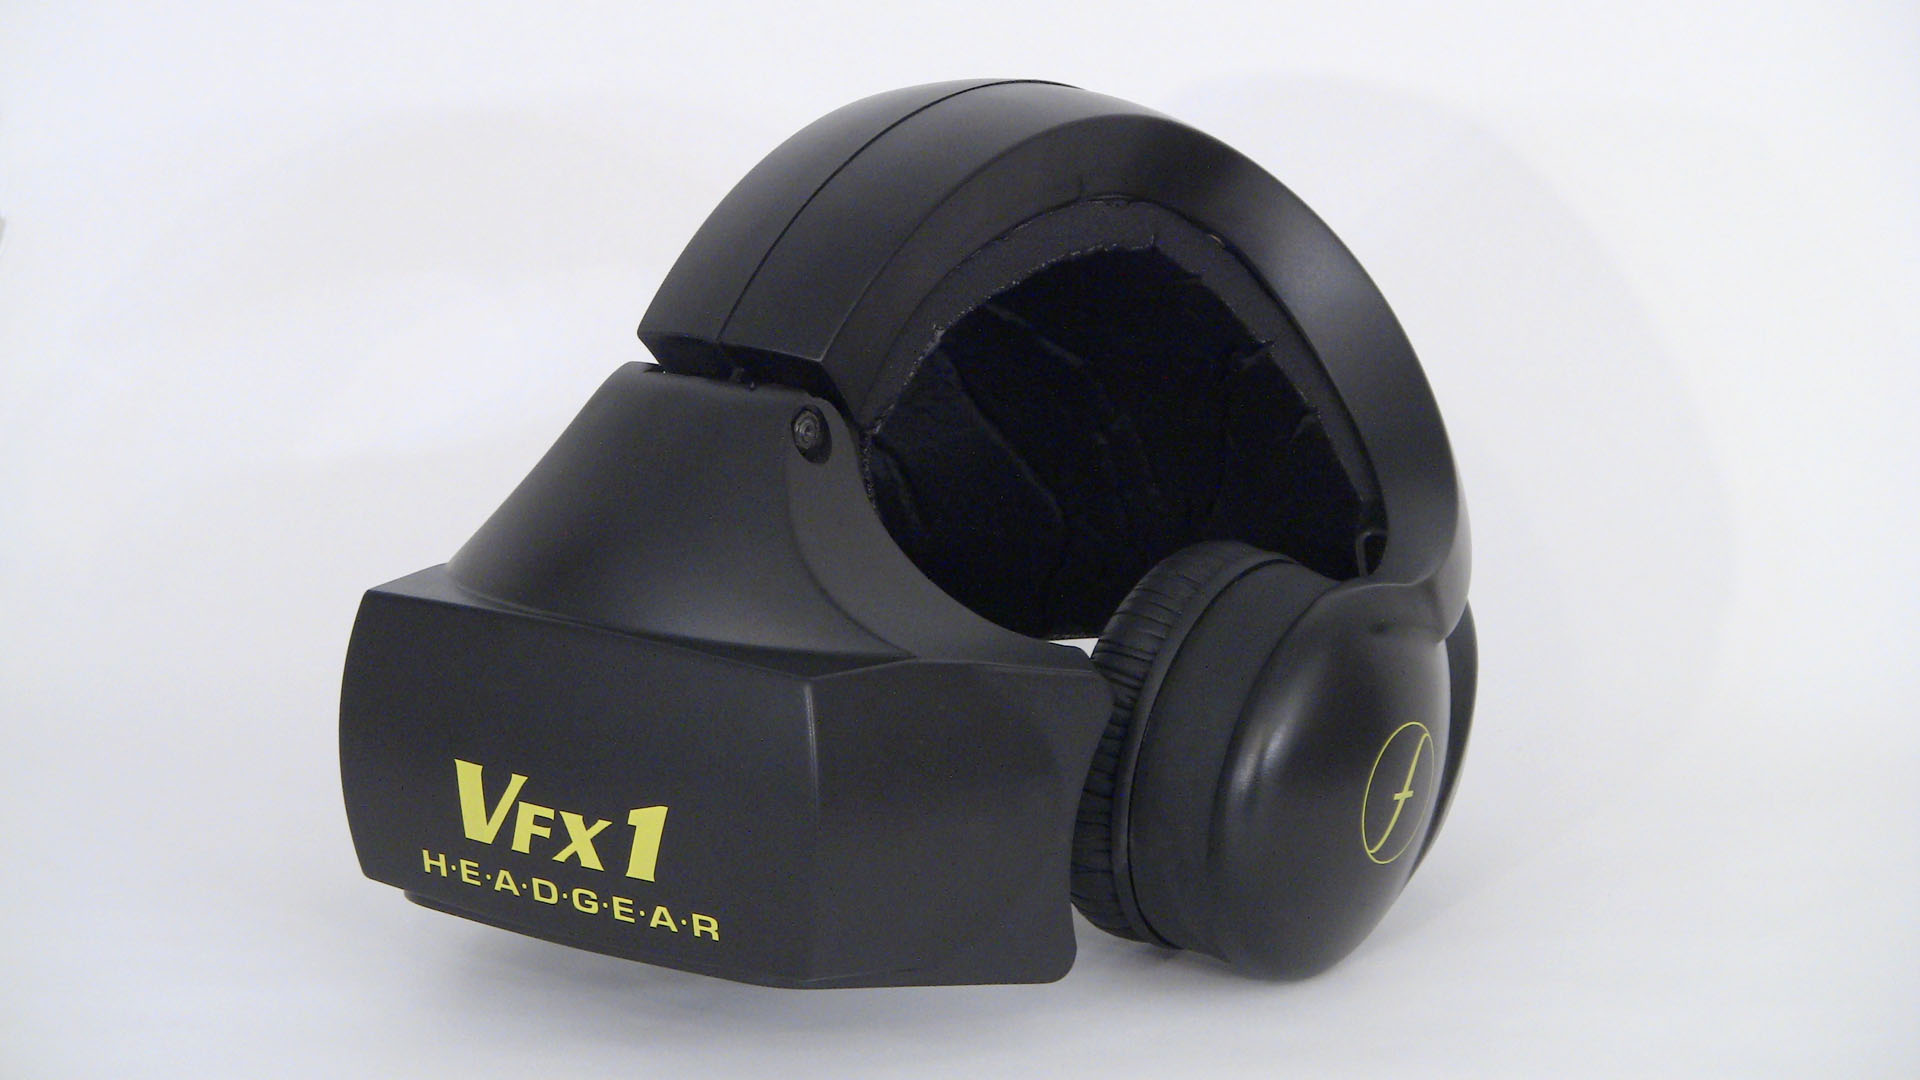
\includegraphics[keepaspectratio,width=\textwidth]{obrazky/vfx1}
	\captionof{figure}{VFX1 headgear}
\end{figure}

Za první komerční headset se dá považovat VFX1. Byl prodáván v devadesátých letech. Skládal se z helmy, ovladače a ISA karty.

Tento headset měl dva LCD displeje s rozlišením 263x230 a zorný úhel 45$ ^{\circ} $.\cite{vfx1}

\subsubsection{HTC Vive}

\begin{figure}
	\centering
	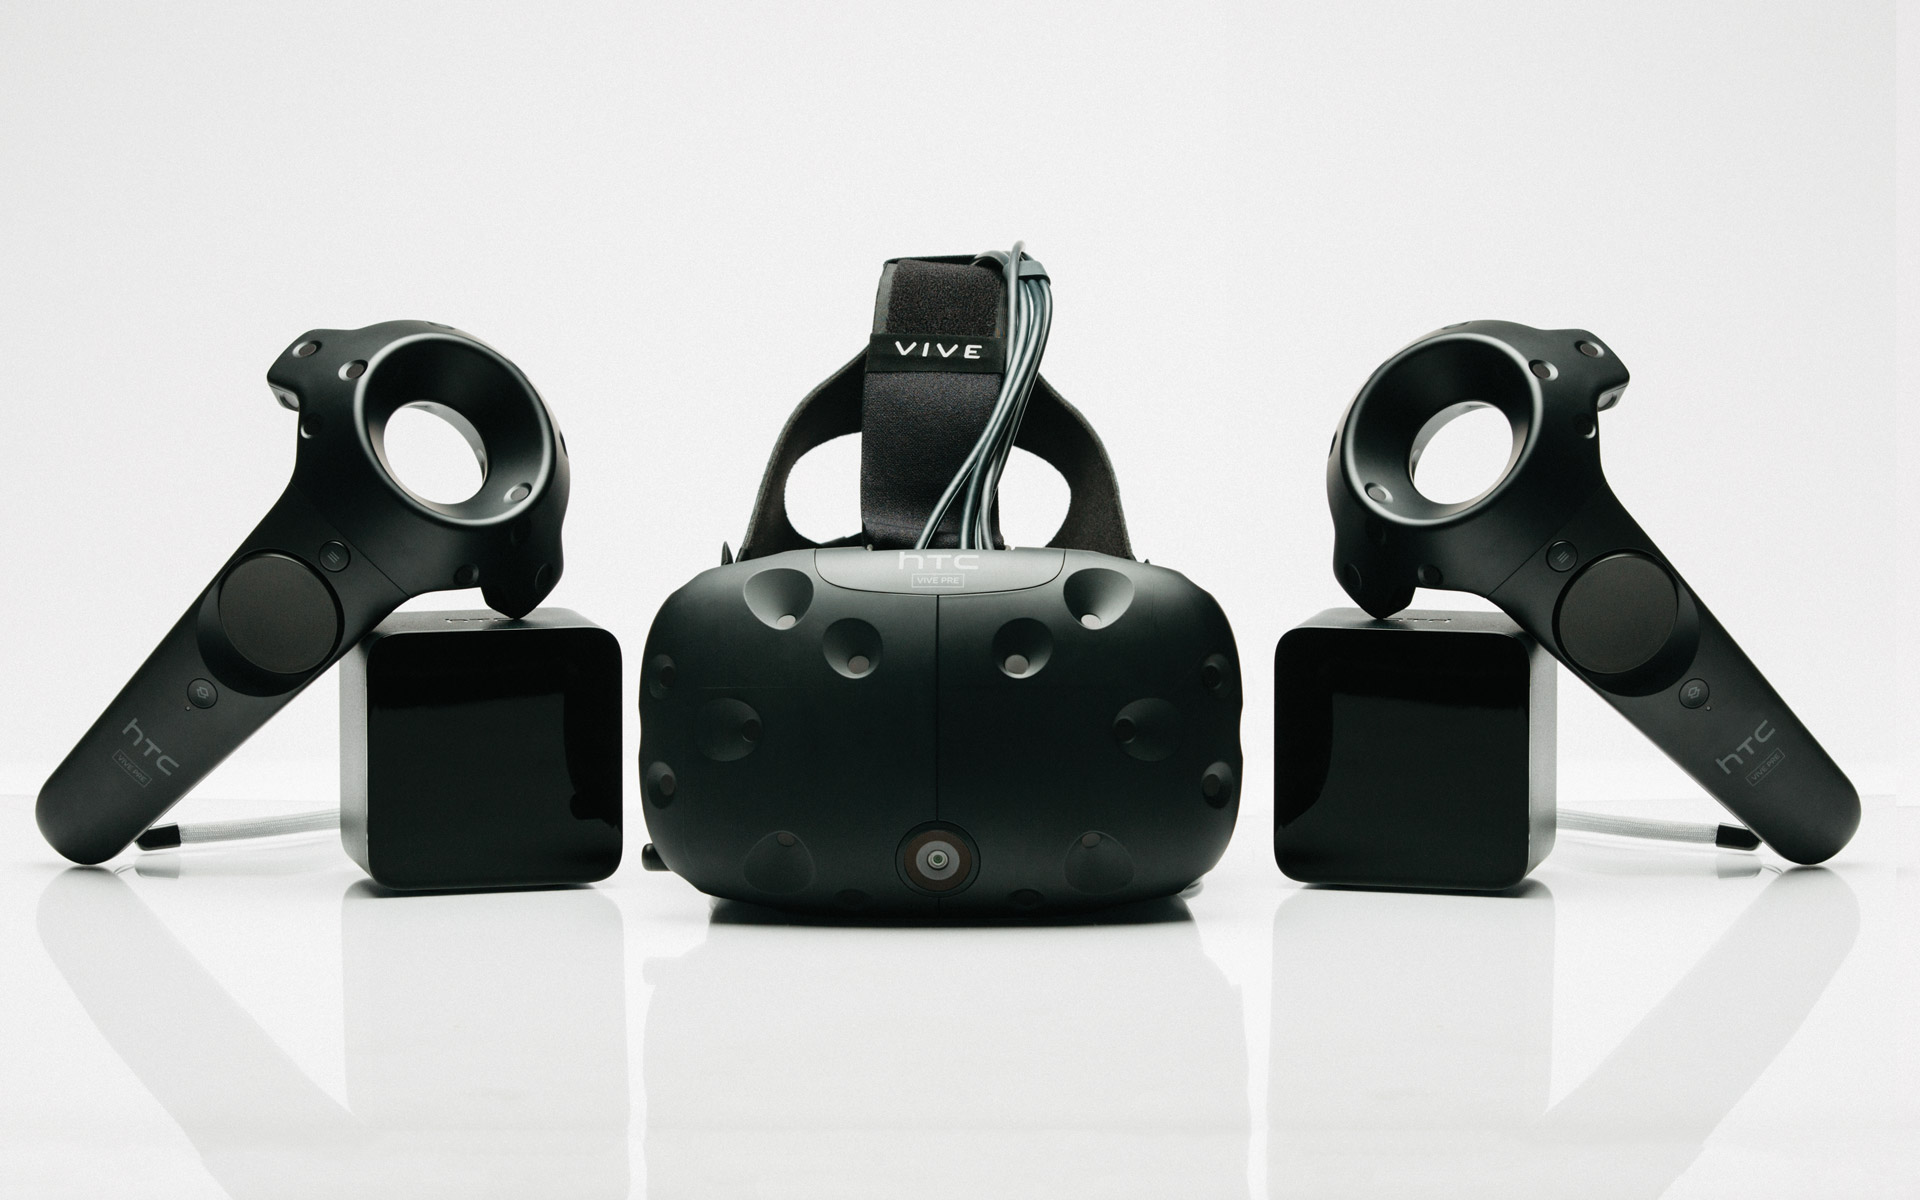
\includegraphics[keepaspectratio,width=\textwidth]{obrazky/vive}
	\captionof{figure}{HTC Vive}
\end{figure}

HTC Vive je headset pro virtuální realitu, vyvinut firmou HTC a Valve Corporation, byl vydán 5. dubna 2016. Tato sada obsahuje headset, dva prostorově sledované ovladače a dva snímače polohy. Uživatel se může pohybovat po místnosti velikosti 4.6\jedn{m} na 4.6\jedn{m}.\cite{vive_bbc}


HTC Vive využívá dva displeje s rozlišením 1080x1200\cite{vive_gamespot} a obnovovací frekvencí 90Hz. Zařízení používá více než 70 senzorů jako jsou gyroskopy, akcelerometry a laserové snímače.\cite{vive_bbc}\cite{vive-lasery} Kamera na přední straně headsetu pomáhá identifikovat objekty před uživatelem a zabrání tak kolizi.

Tento headset je podporován platformou SteamVR, vyvíjenou společností Valve Corporation.

\subsubsection{Oculus Rift}

\begin{figure}
	\centering
	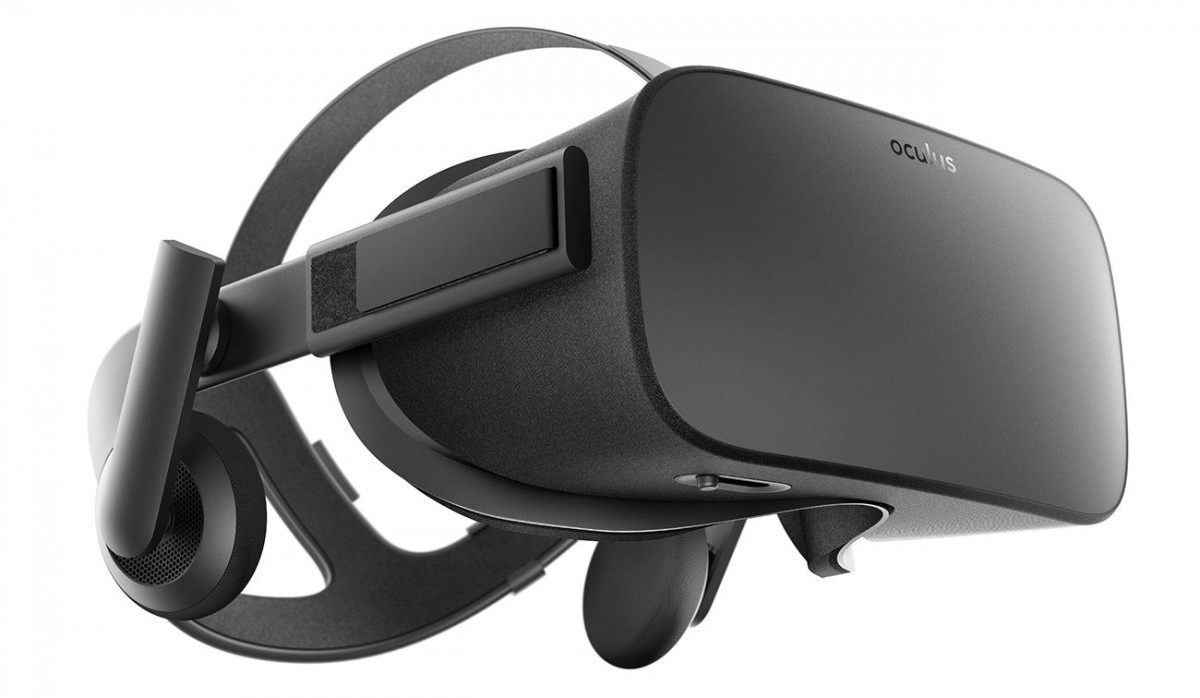
\includegraphics[keepaspectratio,width=\textwidth]{obrazky/oculus}
	\captionof{figure}{Oculus Rift}
\end{figure}

Oculus Rift je headset od společnosti Oculus VR, vydaný 28.3.2016.

Oculus Rift používá dva displeje s rozlišením 1080x1200, obnovovací frekvencí 90Hz a zorným úhlem 110$ ^{\circ} $.\cite{oculus_rift}. Navíc má zabudovaná i sluchátka. Pozice je sledována kromě akcelerometrů a gyroskopů také pomocí stacionární IR kamery, která snímá IR světla na headsetu a kompenzuje chyby inerciální jednotky v headsetu.

Oculus Rift je podporován Oculus Runtime a Steam VR.

\section{Možnosti programování zařízení pro VR}

Všecha tato zařízení pro svou funkci vyžadují, aby daný program s nimi komunikoval pomocí speciálního API.

Současný trh je velmi roztříštěný, každý výrobce headsetu má vlastní API a runtime, navzájem nekompatibilní. Tuto situaci se snaží zlepšit Valve, které vyvinulo OpenVR API primárně pro Vive a nabádá ostatní výrobce, aby dodali podporu jejich zařízení. OpenVR již podporuje Oculus, Vive a OSVR.

Jako další ohlásila vývoj jednotného API organizace Khronos, jejímž cílem je vyvinout API, které nahradí API všech výrobců a tím ulehčí práci vývojářů aplikací. Zároveň by se i zlevnil vývoj aplikací a rozšířil se okruh potenciálních zákazníků.  Valve již ohlásila, že do tohoto projektu předává své rozhraní OpenVR. \cite{khronos_vr}

Já mám k dispozici Vive a Oculus, výběr mých možností se proto zúží na:


\begin{itemize}
	\item Unity 3D, což je multiplatformní herní engine vyvinutý společností Unity Technologies. Tento engine podporuje všechny současné headsety. 
	
	\item Unreal Engine, multiplatformní herní engine vyvinutý společností Epic games. Tento engine podporuje všechny současné headsety.	
	
	\item Použít OpenVR C++ API a naprogramovat si vlastní aplikaci od základu.
\end{itemize}

Herní engine ulehčuje práci vývojářům, protože za ně řeší základní funkce všech her, např. kolize objetků, grafické efekty a v našem případě řeší i přístup k headsetu, tím pádem se mohou zaměřit více na samotný obsah hry. Na herní engine jsou kladeny jiné nároky, než na mou aplikaci. Geometrická náročnost modelu je u většiny her je podstatně menší než u mračna bodů, které potřebuji zpracovávat já. Naopak využívají fotorealistické efekty, mapř. různé odlesky, efekty osvětlení, které já nevyužiju.
Herní engine neobsahují algoritmy, které se využívají při práci s mračny bodů. Případné rozšíření funkcionality by bylo velmi náročné. Enginy používají vysokoúrovňové skriptovací jazyky, které nejsou primárně optimalizovány pro rychlost. Takže by se mohlo stát, že v případě přidávání dalších funkcí bych mohl narazit na limity schopností těchto enginů.
Dalším problémem by mohlo být přidávání knihoven. 
Herní enginy mají navíc licenční podmínky, které by nás mohly limitovat. Proto jsem zvolil cestu naprogramování vlastního enginu.

%% Vložení souboru 'text/vysledky' s popisem vysledků práce
\chapter{Výběr datového formátu a Implementace programu}

\section{Datový formát}

Existuje velké množství datových formátů pro ukládání mračen bodů, proto nebylo možné se všemi detailně zabývat. Na základě požadavků aplikace vyplynuly následující kritéria:

První kritérium je široká podpora různých programů, které mohou být zdrojem dat pro mou aplikaci. Tím eliminujeme nutnost dalšího programu, který by sloužil pouze k převodu formátu na mnou podporovaný. 

Druhé kritérium je flexibilita formátu. Některé formáty podporují jen pevně dané vlastnosti, což se časem může negativně projevit. 

Třetí kritérium je jednoduchost integrace podpory tohoto formátu. 

\subsection{Textový formát}

Tento formát ukládá všechna data jako text. První řádek těchto formátů je hlavička, která udává jaké vlastnosti a v jakém pořadí v souboru jsou.
Seznam některých vlastností:

\begin{itemize}
	\item X,Y,Z jako souřadnice bodů
	\item R,G,B jako barva bodu v rozsahu 0 až 255
	\item Rf,Gf,Bf jako barva bodu v rozsahu 0 až 1
	\item Nx,Ny,Nz jako vektor normály bodů
\end{itemize}

Některé formáty mají na druhém řádku údaj o počtu bodů v souboru. Jednotlivé body jsou pak v souboru odděleny novým řádkem. Tento formát bodů je široce rozšířený. Existuje několik variací tohoto formátu, většinou ale mají jen malé odlišnosti. Jedna z odlišností je oddělovač sloupců, může to být mezera, tabulátor, čárka nebo středník.  Nevýhodou tohoto formátu je pomalé zpracování a neefektivní ukládání. Je to zatím jediný podporovaný formát mého programu.

\subsection{Stereo Lithography STL}

Tento formát se používá hlavně pro 3D tisk, podporuje pouze povrchovou geometrii objektu bez barvy, textury nebo jiných běžných CAD atributů, proto je pro mračna bodů i meshe nevhodný.

\subsection{Wavefront OBJ}

Tento formát popisuje pouze geometrii objektu, tj. vrcholy, texturovací souřadnice, normály bodů a stěny. Materiály, které popisují vizuální stránku objektu, jsou v externím .mtl souboru. To je soubor, který definuje světloodrazivé vlastnosti pro počítačovou grafiku. Tento formát je nevhodný jak pro mračno bodů, tak pro mesh, protože se při vykreslování zpravidla používá pouze barva.

\subsection{Polygon file format PLY}

Tento datový formát podporuje jak mračna bodů, tak i meshe. Formát také dovoluje uložit vlastnosti jako barvu, normály a také uživatelem definované parametry. Podporuje široké spektrum datových typů: 1 až 4 bytové celočíselné jak znaménkové, tak neznaménkové, a plovoucí řádovou čárku jak v jednoduché, tak ve dvojité přesnosti.

Typický soubor obsahuje seznam vrcholů v x,y,z formátu a seznam stěn jako indexy do seznamu vrcholů.

Struktura tohoto souboru se skládá z hlavičky a vlastních dat.
Hlavička je seznam řádků textu, které popisují data v souboru. Jednotlivé parametry jsou určeny klíčovým slovem \texttt{element}, za nímž následuje popis vlastnosti a seznam vlastností tohoto elementu. Tyto jsou pak uvedeny klíčovým slovem \texttt{property} za nímž následuje jeho datový typ a název.

Je široce podporován (Blender, CloudCompare \dots) a je rozšiřitelný. Existuje ve dvou verzích, binární a textové.\cite{ply_format}

\subsection{Point Cloud Data}

Tento formát vznikl jako součást Point Cloud Library\cite{pcl}\cite{pcl_icra}. Existuje v textové i binární verzi. Jeho textová verze má velmi podobnou strukturu jako ostatní textové formáty.

Jeho hlavní výhoda je podpora organizovaných mračen. To jsou mračna, jejichž body představují nejaký obraz nebo matici, kde se data rozdělují na řádky a sloupce. Příklady takovýchto mračen jsou například data z TOF kamer. Výhoda spočívá ve znalosti vztahů mezi sousedními body, čímž se zrychlí operace s nejbližšími body.

Integrace tohoto formátu je jednoduchá, protože by se využila celá knihovna knihovna.

\subsection{Finální výběr}

Z výše uvedených datových formátů se mi jeví jako nejlepší datový formát PLY, protože podporuje jak mračna, tak meshe a podporuje vlastní parametry.

\section{Engine}

Tento engine je napsán v C++ a jsou používány pouze svobodné knihovny. Aplikace je koncipována jako multiplatformní, momentálně je schopná běžet na PC s OS Microsoft Windows a GNU/Linux.

Aby se engine dal spustit i pod OS GNU/Linux, musel jsem ako 3D API  použít OpenGL\cite{opengl}, v mém případě ve verzi 3.3 Core Profile. Pro kontrolu funkcí OpenGL za běhu, používám knihovnu The OpenGL Extension Wrangler Library \cite{glew}. Tato knihovna je pod modifikovanou BSD licencí\cite{glew-lic}, Mesa 3-D licencí\cite{mesa3d-lic} a Khronos licencí\cite{khronos-lic}.  Pro vytvoření okna, kontextu a snímání uživatelského vstupu je použita knihovna GLFW\cite{glfw3} verze 3, tato knihovna je pod licencí zlib/libpng\cite{zlib-libpng}.

\subsection{Požadavky virtuální reality}

Protože je engine primárně určen pro vykreslování ve virtuální realitě, jsou na něj kladeny jisté požadavky. Aby vjem virtuální reality nebyl rušivý nebo dokonce nepříjemný je nutné dodržet dostatečnou snímkovací frekvenci a velmi krátkou odezvu na povely operátora. Proto je nutné se věnovat výkonové optimalizaci.

\subsection{Vykreslování bodů}

Nejprve bylo nutné vyřešit způsob vykreslení bodů. Pokud je budeme vykreslovat jako body s nějakou velikostí, budou na kameru vždy natočeny kolmo a budou mít vždy stejnou velikost nehledě na vzdálenost od kamery a to bude mít negativní dopad na výsledný vjem operátora. Proto jsem se rozhodl vykreslovat je jako malé krychle. To vyřeší problém hloubky obrazu a zlepší výsledný vjem, za cenu zvýšeného počtu.

Nejjednodušší způsob vykreslení krychle je vykreslovat každou stěnu zvlášť.

Místo kreslení čtyřúhelníku se ale kreslí po dvou trojúhelnících, protože u trojúhelníků jsou všechny body vždy v rovině a toto může ovlivnit osvětlení. Další problém čtyřúhelníků je problematická lineární interpolace mezi jednotlivými body, což negativně ovlivní obarvení nebo otexturování. Takto se počet vrcholů zvýší 36 krát.

Teoreticky je rychlost vykreslování velmi závislá na počtu vrcholů a proto jsem začal uvažovat o optimalizaci. Pokud se budou krychle vykreslovat maximálně optimalizované, pomocí dvou trojúhelníkových vějířů, tak se počet vrcholů pouze zšestnáctinásobí. V tom případě se ale musíme vzdát normál, které se používají pro simulaci osvětlení, protože v případě krychle je jeden vrchol společný pro tři stěny tudíž jsou potřeba 3 normály na vrchol. Pokud se normál nechceme vzdát, musíme každou stěnu kreslit odděleně, což lze dvěma způsoby. První a jednodušší je aktuální stav. Druhý způsob je kreslení stěn jako trojúhelníkového pruhu, kde počet vrcholů naroste 24 krát.

Tuto teorii jsem se pokusil experimentálně ověřit. Výsledek byl opačný od očekávání. V případě nulové optimalizace se testovací scéna vykreslovala zhruba 117 snímků za vteřinu, v případě trojúhelníkových pruhů zhuba 63 a v případě vějířů 98. Přesné vysvětlení pro toto nemám, nicméně všechny zmínky na internetu naznačují\cite{tri_opt_1}\cite{tri_opt_2}, že by mohlo jít o optimalizaci na úrovni hardwaru grafických karet.

\subsection{Omezení procesorové zátěže}

Dále je nutné omezit veškterá OpenGL volání, protože jejich režie je nezanedbatelná. Proto je nutné se vyhnout všem zastaralým technikám vykreslování. Pokud bych například vykresloval bod po bodu v cyklu byl by zatěžován procesor mnohem více než grafická karta a výkon by byl velmi nízký. Proto je nutné využívat prvky jako Vertex Buffer Object\cite{vbo} a Vertex Array Object\cite{vao}.

Protože se krychle skládá z více vrcholů některé vlastnosti, jako barva či skalární pole, by se pro každý vrchol opakovali. Toto opakování jsem eliminoval geometrickým instancováním. Je to způsob jak nakreslit mnoho opakujících se objektů (body ve formě krychlí) s lišícími se parametry (pozice, barva). Do paměti grafické karty se načte pouze jedna krychle a pak seznam pozic, barev popřípadě dalších parametrů. Postupně se pak pro všechny parametry v seznamu kreslí krychle.

\subsection{Podporovaný formát}

Kvůli jednoduchosti jsem na začátku implementoval pouze omezenou podporu textového formátu. Počáteční implementace byla velmi jednoduchá ale také velmi pomalá. Testovací soubor 50 milionů řádků na i7-6700k při taktu 4.5\jedn{GHz} trval načíst 78.3\jedn{s}. Doba načítání souboru mě brzdila při vývoji, protože jsem musel při každém spuštění čekat na načtení souboru. Toto vyústilo v optimalizaci.

Původní implementace využívala pro čtení \texttt{std::ifstream}, řádky se načítaly v cyklu pomocí \texttt{std::getline} a pomocí \texttt{std::stringstream} a operátoru \texttt{>>} se jednotlivé sloupce přímo převáděly na \texttt{float}. Všechna data se pak ukládala do \texttt{std::vector}.

Pak jsem si ověřil že značnou část času trvá převod řetězce na \texttt{float}. Když jsem přestal převádět na \texttt{float} a nechával jednotlivé čísla v řetězci doba se zkrátila na 44.8\jedn{s}.

Při pátrání na internetu jsem našel několik zmínek o tom že C funkce jsou obecně rychlejší.

Konečná implementace je téměř v čistém C. Nejprve se ze souboru do paměti načte blok dat o aktuálně nastavené hodnotě v programu, ten se poté v cyklu dělí na řádky pomocí \texttt{strchr} a tento řádek se pak ve vnořeném cyklu dělí na jednotlivé čísla pomocí \texttt{strtok}. Tyto čísla se ukládají v řetězci do dvourozměrného pole. Jakmile se v bloku nenajde další prázdný řádek, tak se k tomuto bloku přidá dálší načtený blok. Poté se spustí paralelně na ostatních jádrech procesoru konverze řetězců na \texttt{float} a zároveň se v hlavním vlákně rozděluje aktuálně načtený blok. Této implementaci trvá na stejném PC načíst stejný soubor pouze 43.9\jedn{s}.

\subsection{Segmentace mračna}

Mračna, která mají přes jeden milion bodů, jsou příliš náročná na vykreslování, proto je nutné sáhnout po optimalizaci. Velmi často není celé mračno viditelné na obrazovce. Díky tomu lze využít tzv. frustum culling\cite{frustum-culling}, což je technika, která nám umožnuje zjistit, které objekty, nejsou v záběru pohledu, tudíž není nutné je vykreslovat. Aby toto bylo možné je nutné mračno rozdělit na segmenty. Při segmentaci se mračno rozdělí do tzv. octree, což je datová struktura, kde každý uzel má právě 8 potomků. To se velmi hodí při rozdělování třírozměrných objektů, kde se objekt rozdělí na poloviny podle všech rozměrů. Rozděluje se podle počtu bodů v jednom segmentu, pokud je v segmentu víc bodů, než aktuálně v programu nastavená hodnota, segment se rozdělí na 8 podsegmentů. Toto se provádí rekurzivně pro všechny segmenty.

\subsection{Grafické rozhraní}

Samotné OpenGL umí jen vykreslovat základní tvary a také nemá žádnou podporu vykreslování písem. Toto dělá tvorbu grafického rozhraní poměrně složitou a to beru v úvahu pouze vzhled. Jakákoli funkčnost tohoto rozhraní už jde mimo OpenGL úplně.

Existuje řada knihoven, které tuto funkcionalitu doplňují. Většina jsou buď neznámé malé neudržované projekty a nebo velmi komplexní knihovny, které naopak příliš zasahují do samotné funkčnosti zbytku programu.

Vybrat vhodnou knihovnu je velmi obtížné, protože pro zhodnocení knihovny je nutné si ji vyzkoušet což je časově náročné a informace na internetu nehodnotí příliš objektivně.

Pro tento demonstrační program jsem se rozhodl naimplementovat vlastní jednoduché grafické rozhraní.

\subsection{Zobrazení mračna}

\subsubsection{Změna velikosti bodů}

Mračna mají různé hustoty bodů. Aby mračno nebylo příliš řídké nebo se naopak body nepřekrývaly, bylo nutné implementovat změnu velikosti těchto bodů.

Velikost bodů se mění skokově podle funkce $ 2^n $, kde n je celé číslo viz obrázek \ref{velikosti}. Počáteční hodnota tohoto čísla je $ -8 $.

\subsubsection{Zobrazení skalárního pole}

Některá mračna mají uloženo tzv. skalární pole. To znamená, že ke každému bodu je přiřazeno číslo. Toto číslo má po domluvě nějaký význam, například teplota.

Aby se dalo toto pole zobrazit je nutné ho převést na barevnou škálu. Já ho převádím tak že celý rozsah tohoto pole upravím na rozsah 0 až 120. Tuto hodnotu poté použiji jako odstín HSV barevného modelu s maximální sturací a hodnotou. Tuto barvu pak převedu do RGB jakodruhou možnou barvu bodu.

Tuto výslednou barvu lze poté prolínat s originální barvou podle alpha blendingu\cite{alpha-blending} viz obrázek \ref{skalar}.


\begin{figure}
	\centering
	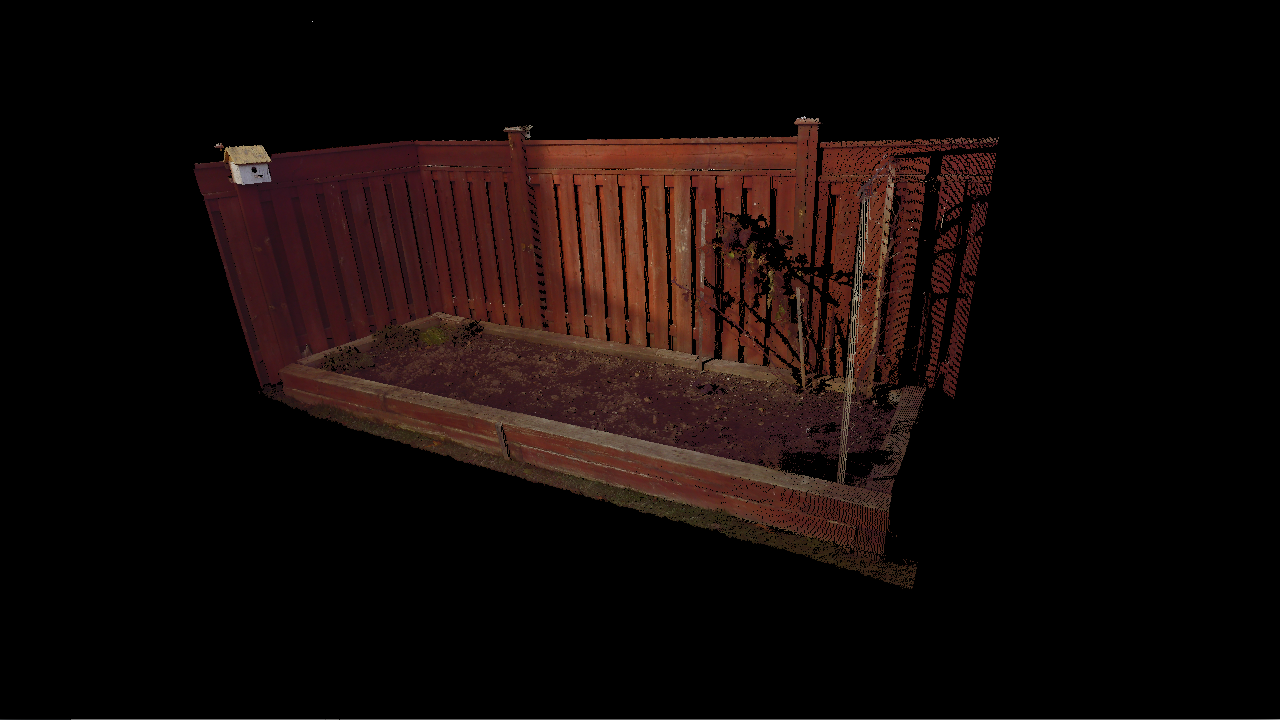
\includegraphics[keepaspectratio,width=\textwidth]{obrazky/mrak}
	\captionof{figure}{Pohled na načtené mračno}
	\label{mrak}
\end{figure}

\begin{figure}
	\centering
	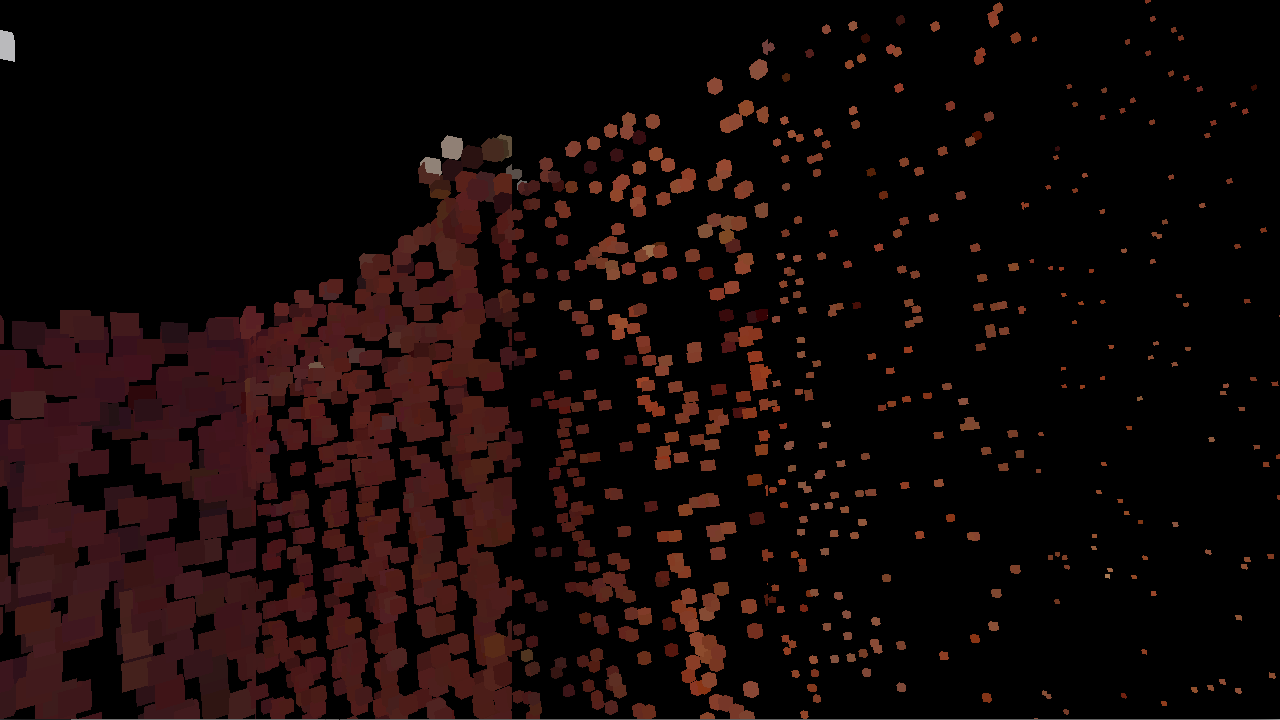
\includegraphics[keepaspectratio,width=\textwidth]{obrazky/velikosti}
	\captionof{figure}{Demonstrace změny velikosti bodů}
	\label{velikosti}
\end{figure}

\begin{figure}
	\centering
	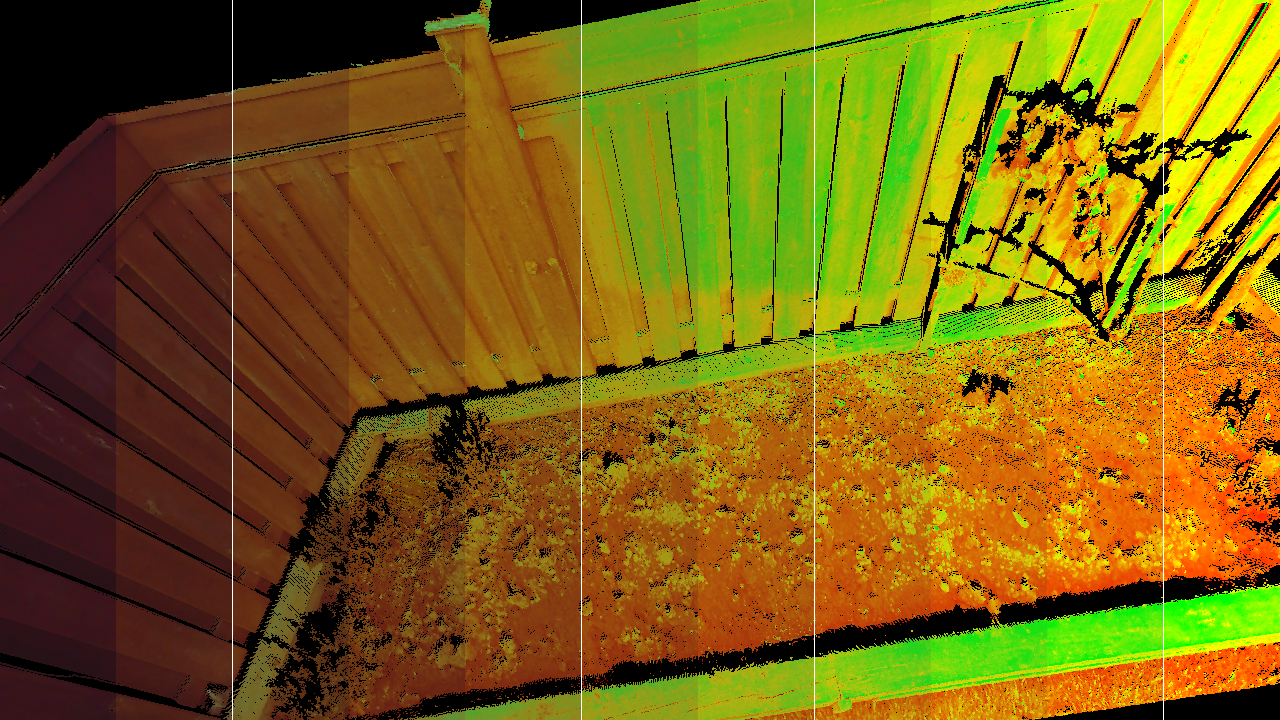
\includegraphics[keepaspectratio,width=\textwidth]{obrazky/skalar}
	\captionof{figure}{Demonstrace přimíchávání škály skalárního pole}
	\label{skalar}
\end{figure}

\FloatBarrier

\section{Ovládání programu}

Veškeré ovládání programu bylo nejprve implementováno pomocí klávesnice.

Pomocí kláves W a S se pohled posouvá po ose Z, A a D po ose X a Alt a mezerník po ose Y. Pomocí šipek nahrou a dolů se pohled natáčí podle osy X, pomocí šipek doleva a doprava podle Y a pomocí kláves Q a E se naklápí podle osy Z.

Klávesou R se velikost bodu zdvojnásobí, klávesou F sníží na polovinu. Klávesami T a G se plynule přechází mezi barvou mračna a skalárním polem.

Klávesou M se vyvolá menu. Šipkami nahoru a dolů se vybírají jednotlivé prvky v menu, výběr se potvrdí klávesou Enter, pro vrácení o úroveň nahoru klávesa Escape.

Program se uzavře stisknutím Escape mimo menu.

\begin{figure}
	\centering
	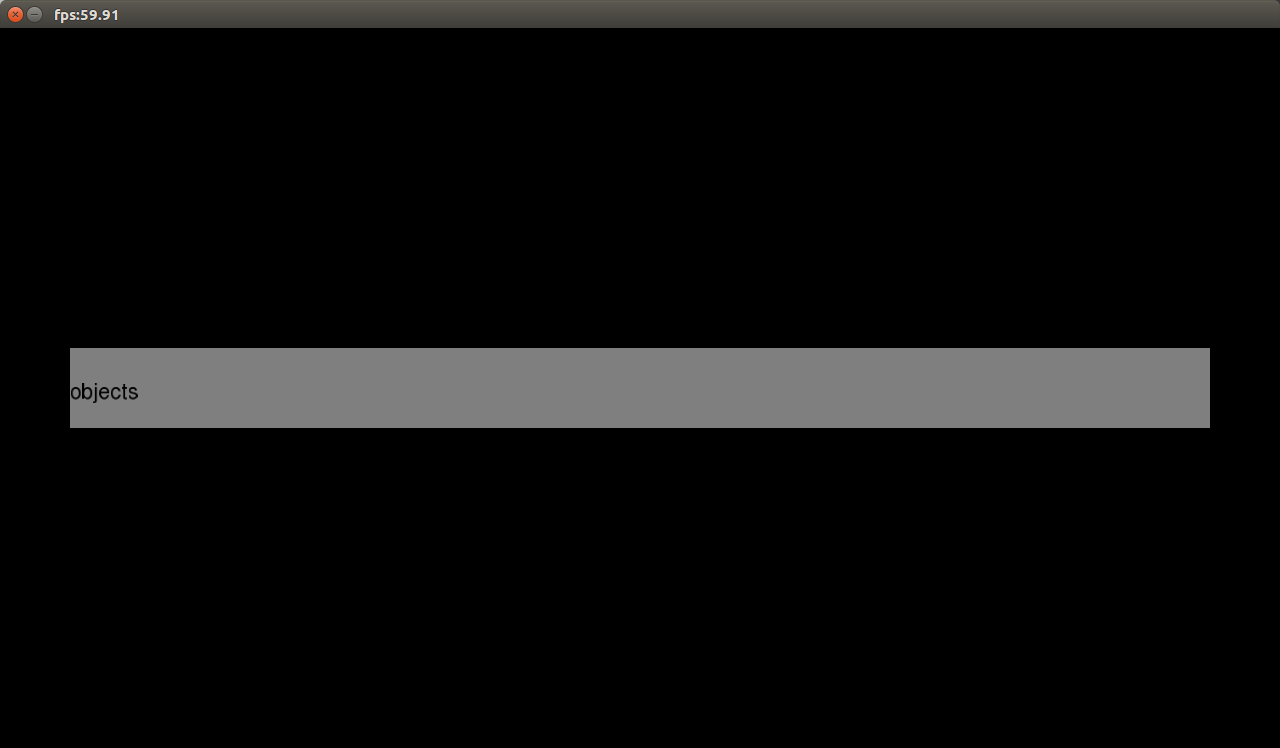
\includegraphics[keepaspectratio,width=\textwidth]{obrazky/objects}
	\captionof{figure}{Hlavní menu}
	\label{hlavni-menu}
\end{figure}

\begin{figure}
	\centering
	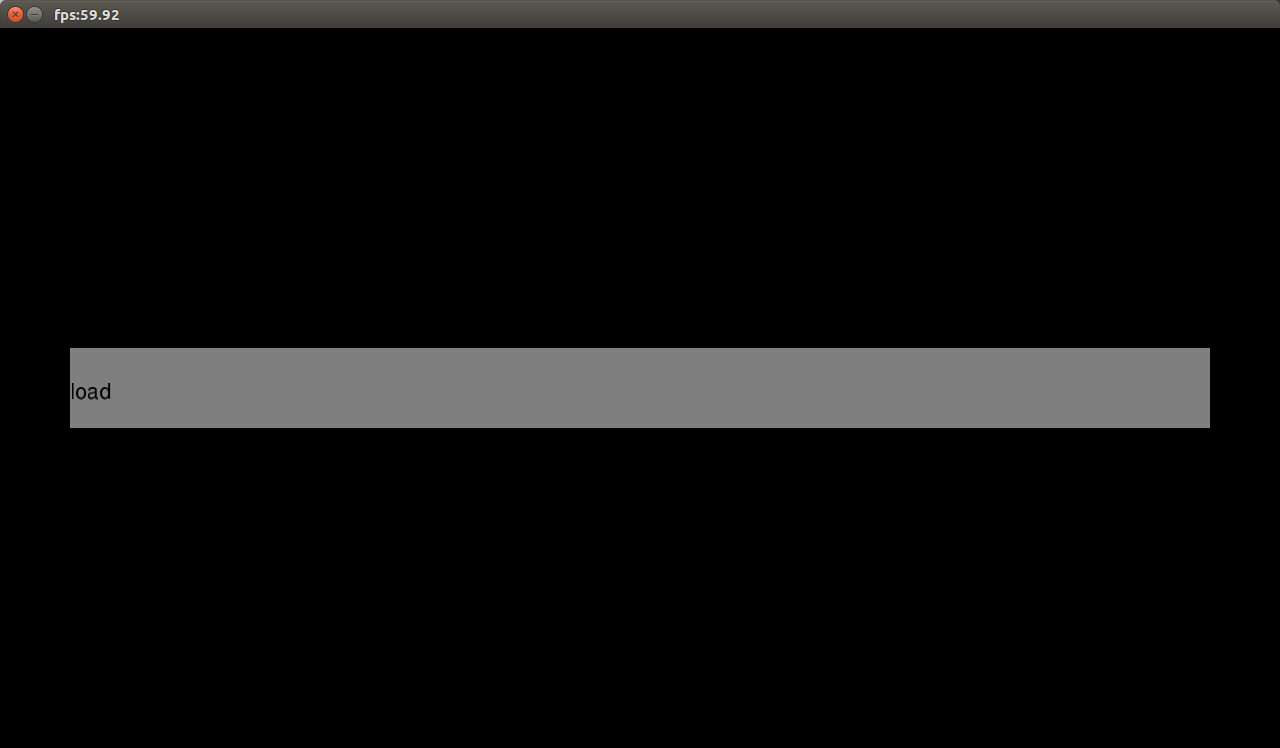
\includegraphics[keepaspectratio,width=\textwidth]{obrazky/prazdne-objekty}
	\captionof{figure}{Menu objekty}
	\label{objects}
\end{figure}

Po vyvolání menu lze vidět položku objects, viz obrázek \ref{hlavni-menu}, v ní je seznam všech načtených mračen do programu a položku load (obrázek \ref{objects}), pomocí ní lze načíst mračno. Pokud operátor vybere již načtené mračno, bude mít v nabídce možnost toto mračno odstranit.

Poté jsem implementoval částečné ovládání pomocí pravého ovladače.

Pro pohyb po scéně je nejprve nutné stisknout trigger, poté táhnout ovladačem a nakonec trigger uvolnit. Stisknutím horního tlačítka na pravém ovladači se vyvolá menu. Pohybem prstu po trackpadu se posouvá položkami v menu, triggerem se výběr potvrdí. Horním tlačítkem se také vrací na vyšší úroveň menu a menu uzavírá.




%% Vložení souboru 'text/zaver' se závěrem
\chapter{Závěr}

Jako datový formát jsem vybral PLY, pro svou flexibilitu. V případě, že by se využila funkcionalita Point Cloud library by se využil i formát PCD.

Aplikace svůj demonstrační účel splnila. Lze načítat nekolik mračen bodů, pohybovat se v prostoru, měnit velkosti bodů a zobrazit skalární pole. Hardwarové nároky počítače jsou závislé pouze na složitosti načteného mračna.

Pro další vývoj aplikace bude vhodné přehodnotit celkový návrh a vybrat vhodnou knihovnu pro grafické rozhraní, aby bylo možné implementovat lepší uživatelské rozhraní, díky kterému bude možné pohodlné ovládání po přidání dalších funkcí a také získat uživatelskou zpětnou vazbu pro zkvalitnění 

Další vylepšování by se mohlo týkat výkonu. Pro virtuální realitu se musí vykreslovat vždy dva nezávislé snímky. Tyto snímky by mohly vykreslovat dvě grafické karty. V tomto by velmi pomohlo použití nových API jako je Vulkan nebo DirectX12, které jsou na tuto situaci lépe navrženy než předchozí API.


%% Vložení souboru 'text/literatura' se seznamem literatury
%\bibliographystyle{csplainnat}
%\bibliographystyle{plain}
\bibliographystyle{czechiso}

\bibliography{dokumentace}

%% Vložení souboru 'text/zkratky' se seznam použitých symbolů, veličin a zkratek
%\begin{seznamzkratek}{KolikMista}

	\novazkratka{zkTemp}		% název
		{Velikost levého sloupce seznamu}								% zkratka
		{-- určujete délkou parametru prostředí \texttt{seznamzkratek} (viz zdroják)}
											% rozvinutí zkratky

	\novazkratka{zkDSP}		% název
		{DSP}								% zkratka
		{číslicové zpracování signálů -- Digital Signal Processing}
											% rozvinutí zkratky
	%%% bsymfvz
	\novazkratka{symfvz}						% název
		{\ensuremath{f_\textind{vz}}} % symbol
		{vzorkovací kmitočet}					% popis
	%%% esymfvz

\end{seznamzkratek}


%% Začátek příloh
%\prilohy

%% Vysázení seznamu příloh
%\seznampriloh

%% Vložení souboru 'text/prilohy' s přílohami
%\include{text/prilohy}

%% Konec dokumentu
\end{document}
